\documentclass{report}
\usepackage[utf8]{inputenc}

% Títulos automáticos en español
\usepackage[spanish]{babel}

% Soporte para buenas urls e hipervínculos entre secciones
\usepackage{hyperref}

% Citas y referencias en formato APA
% Si quiere las citas y referencias en IEEE comente esta línea
\usepackage{apacite}

% Imágenes y figuras
\usepackage{graphicx}

% Código fuente con números de línea
\usepackage{listings}
% Puede cambiar el lenguaje de código fuente
% https://www.overleaf.com/learn/latex/code_listing#Supported_languages
\usepackage{multirow}


\lstset{
    language=C,
    basicstyle=\footnotesize,
    numbers=left,
    stepnumber=1,
    showstringspaces=false,
    tabsize=1,
    breaklines=true,
    breakatwhitespace=false,
}


\def \unidad{Nombre de la escuela o unidad}
\def \programa{Nombre del programa o carrera}
\def \curso{Código - Nombre del curso}
\def \titulo{Título del Informe}
\def \subtitulo {Subtítulo}
\def \autores{
    Nombre del primer autor\\
    Correo electrónico\\
    Carnet\\
    
    \vspace{0.5cm}
    
    Nombre del segundo autor\\
    Correo electrónico\\
    Carnet
}
\def \fecha{Febrero 2021}
\def \lugar{
    Provincia, 
    Costa Rica
}

% Inicia el documento 
\begin{document}

% Inserta la portada del documento
\begin{titlepage}
    \begin{center}
        \vspace*{1cm}
        
        
\includegraphics[width=0.8\linewidth]{figuras/logo_tec.jpg}\\
        \LARGE
        \unidad\\
        \programa\\
        \curso
        
        \vspace{1cm}
        
        \Huge
        \textbf{\titulo}
            
        \vspace{0.5cm}
        \LARGE
        \subtitulo
            
        \vspace{1.5cm}
        
        \large    
        \autores
            
        \vfill
        
        \lugar\\
        \fecha
        
    \end{center}
\end{titlepage}

\tableofcontents

\chapter{Introducción}\label{intro}

Esta es una plantilla para trabajar documentos formales en \LaTeX para informes de trabajos del ITCR, fue diseñada para el curso Fundamentos de Organización de Computadoras.
Esta plantilla utiliza el formato de citas y referencias de APA usando el paquete apacite.

Las tareas y trabajos universitarios deben entregarse en un formato formal que sigan ciertas reglas de estilo. 
\LaTeX es una buena solución para redactar este tipo de documentos sin preocuparse por la estructura ni el diagramado.

\section{Antecedentes}\label{antecedentes}

El matemático y científico en computación Donald Knuth diseñó TeX en 1978 como una respuesta a la necesidad de la época de redactar documentos formales con lenguaje matemático que los editores de texto de la época no podían solventar. En 1984 Leslie Lamport modificó TeX y creó una serie de comandos y macros más sencillos y con más herramientas. A esta versión Lamport le llamó \LaTeX \cite{lopez18}.


\section{Discusión}
\subsection{Tabla de resultados}
\begin{center}
	\begin{tabular}{|c|c|c|c|}		
		
\hline
\multicolumn{4}{|c|}{Tiempo de Ejecución (milisegundos)} \\
\hline
 Subsistema& \multicolumn{3}{|c|}{Versión} \\
 \hline
 & Serial & Concurrente & Paralelo\\
 \hline
huff(completo) & 5360& 2226 & 2036\\
 \hline
huff(lectura) &  36 & 25 & 19\\
 \hline
 huff(compresión) &  5168 & 1957 & 1681\\
 \hline
 dehuff(completo) & 5189 & 2092 & 1855\\
 \hline
 dehuff(descompresion y escritura) & 5146 & 1968 & 1629\\
 \hline
 
	\end{tabular}
\end{center}

\subsection{Analisis de aceleración}

La ley de Amdahl dice que .... y fue hecha por ....

\begin{displaymath}	
	{T_{m} = {T_{a} \cdot \left((1 - F_{m}) + {F_{m} \over A_{m}}\right)}}
\end{displaymath}

La ley de Amdahl puede reescribirse para obtener el incremento de velocidad del sistema completo. La formula sería la siguiente:

\begin{displaymath}	
	A = {1 \over (1 - F_{m}) + {F_{m} \over A_{m}}}	
\end{displaymath}
Donde:\\
$A$, es la aceleración o ganancia en velocidad conseguida en el sistema completo debido a la mejora de uno de sus subsistemas.\\
$A_{m}$, es el factor de mejora que se ha introducido en el subsistema mejorado.\\
$F_{m} $, es la fracción de tiempo que el sistema utiliza el subsistema mejorado.\\






\chapter{Ejemplos}\label{ejemplos}

\section{Figuras}\label{figuras}
\begin{figure}
    \centering
    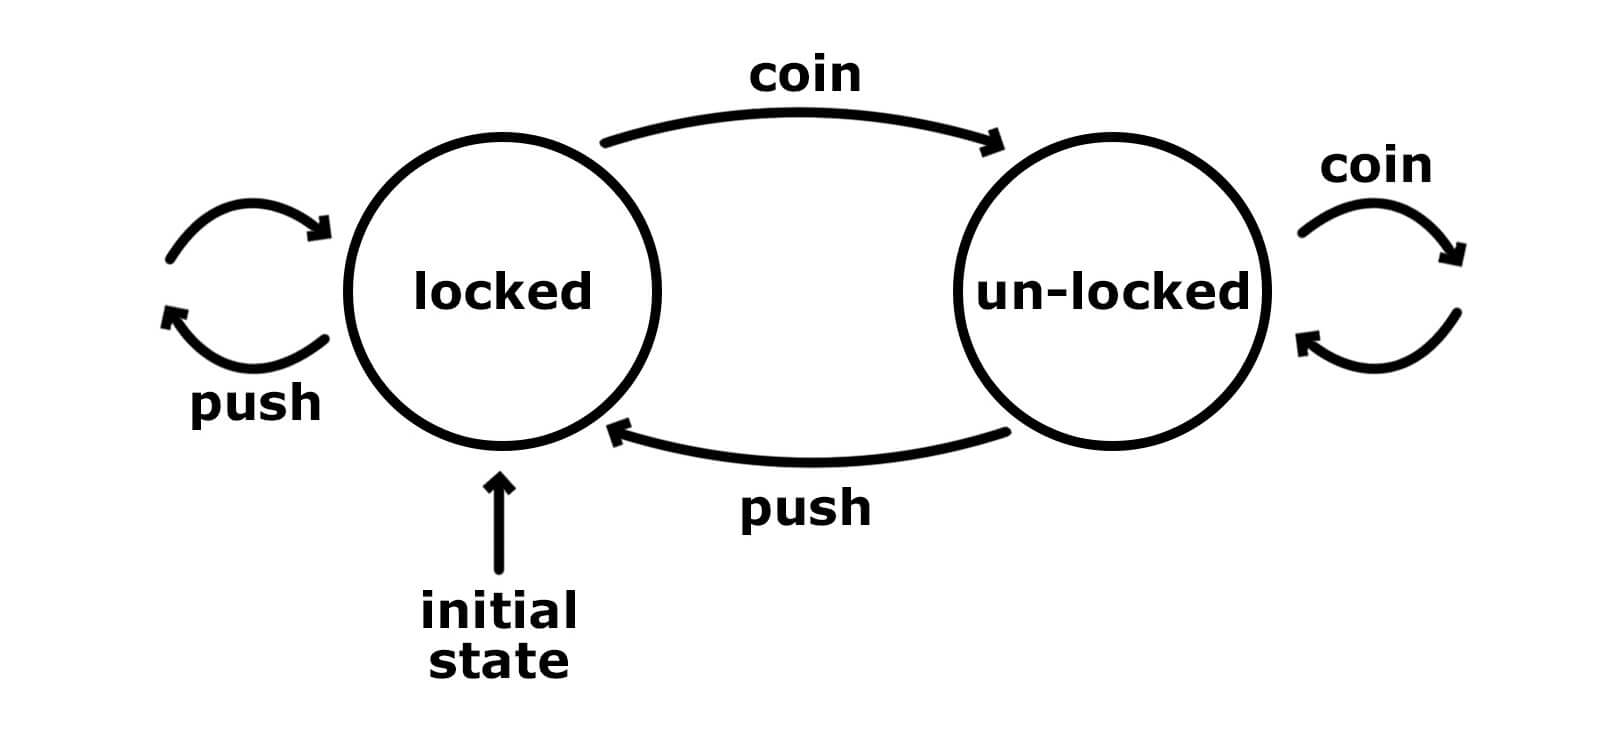
\includegraphics[width=0.8\linewidth]{figuras/maquinaDeEstados.jpg}
    \caption{Ilustración de una máquina de estados finitos}
    \label{fig:msf}
\end{figure}

Las figuras nos permiten ilustrar conceptos de forma más directa. Adicionalmente muchos dominios emplean lenguajes gráficos para representar ciertos principios o procesos. La figura permite incorporar este tipo de herramientas visuales al documento. 
La figura \ref{fig:msf} representa una máquina de estados finitos, nótese como la figura incorpora un texto descriptivo. Este texto es necesario para brindar mejor contexto a la imagen, especialmente cuando no se diagrama junto al texto que acompaña.

\section{Listas y Enumeraciones}\label{listas}

Las listas de viñetas y enumeraciones nos permiten organizar información y secuenciarla de forma visualmente agradable. Bien empleadas las listas pueden ayudar a organizar los datos presentados y establecer cierta noción de jerarquía.

Una lista puede contener solamente algunos elementos simples:
\begin{itemize}
    \item ítem 1
    \item ítem 2
    \item ítem 3
\end{itemize}

Pero también se pueden emplear de formas más complejas e interesantes:

\begin{itemize}
    \item \textbf{Conceptos amplios:} Por ejemplo una lista puede usarse para representar ideas más complejas que pueden organizarse en algún tipo de jeraruía. 
    Una lista de este tipo puede contener mucho texto, párrafos inclusive, y aún así mantener la indentación y estructura lineal que permite expresar la relación como parte de la información transmitida.
    
    Los elementos de la lista se pueden introducir con un encabezado en \textbf{negrita} que permita asociar los conceptos con sus definiciones. Similar a las entradas de un diccionario.
    
    \item \textbf{Contenido multinivel:} Otra aplicación de las listas es que permiten organizar contenido en estructuras jerárquicas. En \LaTeX una lista puede:
    
    \begin{itemize}
        \item Anidarse dentro de otra lista
        \item Mostrando múltiples elementos
        \item Dentro de una estructura jerárquica
        \begin{itemize}
            \item Tan profunda
            \item Como el autor
            \item Lo requiera
        \end{itemize}
    \end{itemize}
\end{itemize}

Por supuesto si podemos hacer listas de viñetas, \LaTeX también nos da la posibilidad de usar enumeraciones:

\begin{enumerate}
    \item Las enumeraciones tienen las mismas propiedades.
    \item La única diferencia es que los ítemes se identifican con números, no con viñetas.
    \item Pero soportan:
    \begin{enumerate}
        \item texto corto
        \item texto largo
        \item multinivel
        \item Inclusive es posible combinar ambas estrategias:
        \begin{itemize}
            \item Enumeraciones con listas adentro
            \item Listas con enumeraciones adentro
            \item Cualquier otra combinación que sea necesaria
            
        \end{itemize}
    \end{enumerate}
\end{enumerate}

\section{Referencias Internas}\label{referencias}
En el capítulo \ref{intro} se explica el propósito del documento y algunos antecedentes. Mientras que el capítulo \ref{ejemplos} se enfoca más en funcionalidades puntuales que pueden ser interesantes de \LaTeX. Como se puede apreciar, una de esas funcionalidades es la capacidad de referenciar internamente contenido, usando los comandos \textit{label} y \textit{ref} es posible citar otras partes del documento. Cualquier elemento numerado con una \textbf{etiqueta} se puede referenciar y \LaTeX usará la numeración correcta para referenciar el elemento donde se cite. Por ejemplo en esta sección se puede citar la figura \ref{fig:msf} o la sección \ref{antecedentes}. Una propiedad muy práctica de esta herramienta, es que combinada con el paquete \textbf{hyperref} permite que el documento se entrelace fácilmente, creando hipervínculos entre las secciones justo donde se referencian.

Nótese que estas son referencias internas. Las citas bibliográficas tienen un comando especial: el comando \textbf{cite}.

\section{Código fuente}
En temas de ingeniería es normal que necesitemos programar de vez en cuando. Para esto \LaTeX brinda funcionalidades para renderizar código fuente con un resultado bastante profesional.
Por ejemplo podemos ver el código fuente de un \textit{Hola Mundo} en el lenguaje de programación C:

\begin{lstlisting}
#include <stdio.h>

int main() {
   
   printf("Hello, World!");
   return 0;
}
\end{lstlisting}

Hay más herramientas para mostrar texto técnico. Por ejemplo el ambiente \textit{verbatim} permite mostrar texto con símbolos que normalmente están reservados para código de \LaTeX. Por ejemplo, estas son las primeras líneas de este documento:

\begin{verbatim}
\documentclass{report}
\usepackage[utf8]{inputenc}

% Títulos automáticos en español
\usepackage[spanish]{babel}

% Soporte para buenas urls e hipervínculos entre secciones
\usepackage{hyperref}
\end{verbatim}

\section{Más}
\LaTeX tiene muchísimas características, tantas que es imposible cubrirlas todas en un sólo documento. Por eso voy a dejar una lista breve de algunos enlaces de interés que podrían ser útiles según el tipo de documento:

\begin{itemize}
    \item \textbf{Tablas:} \\
    \url{https://manualdelatex.com/tutoriales/tablas}
    
    \item \textbf{Bibliografía con Bibtex:}\\
    \url{https://www.overleaf.com/learn/latex/bibliography_management_with_bibtex}
    
    \item \textbf{Expresiones Matemáticas:}\\
    \url{http://metodos.fam.cie.uva.es/~latex/apuntes/apuntes3.pdf}
    
    \item \textbf{Presentaciones de Diapositivas:}\\
    \url{https://www.overleaf.com/learn/latex/beamer}
    
    \item \textbf{Gráficas generadas en \LaTeX}\\
    \url{https://www.overleaf.com/gallery/tagged/charts}    
\end{itemize}

% Estilo de bibliografía APA
% Si quiere usar el estilo IEEE comente esta línea
\bibliographystyle{apacite}

% Descomente esta línea para usar el estilo de bibliografía IEEE
%\bibliographystyle{ieeetr}
\bibliography{referencias}

\end{document}
